\documentclass{standalone}
\usepackage{tikz}
\usetikzlibrary{patterns, positioning}

\begin{document}
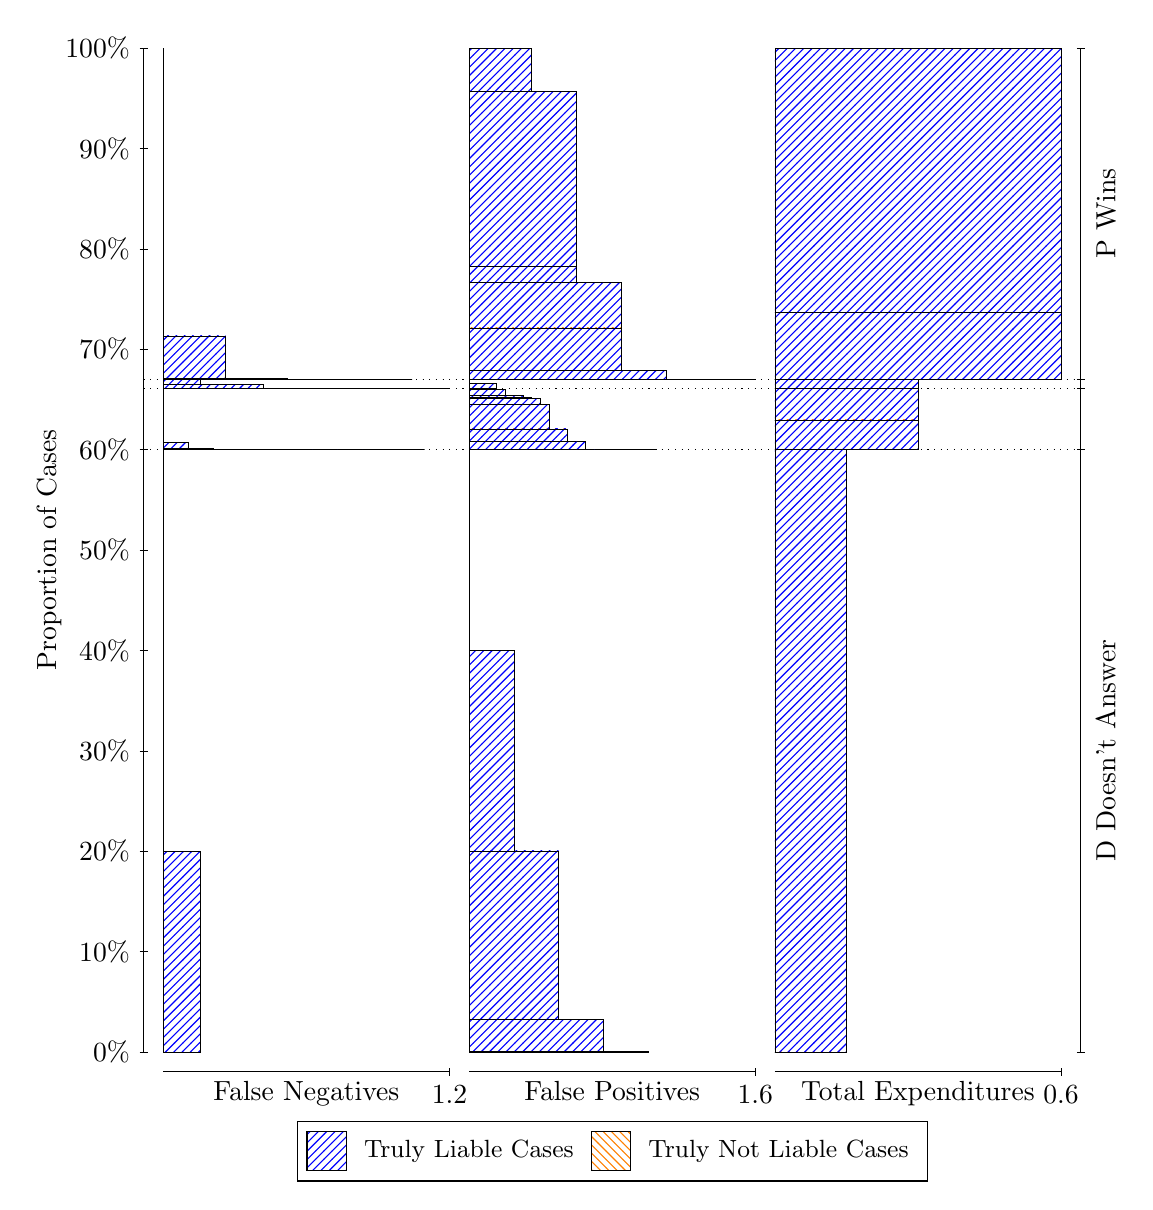
\begin{tikzpicture}
\draw[black, very thin] (1.5,1.75) -- (1.5,14.5);
\node[rotate=90, anchor=center] at (0.3, 8.125) {Proportion of Cases};
\draw[black, very thin] (1.45,1.75) -- (1.55,1.75);
\node[anchor=east] at (1.45, 1.75) {0\%};
\draw[black, very thin] (1.45,3.025) -- (1.55,3.025);
\node[anchor=east] at (1.45, 3.025) {10\%};
\draw[black, very thin] (1.45,4.3) -- (1.55,4.3);
\node[anchor=east] at (1.45, 4.3) {20\%};
\draw[black, very thin] (1.45,5.575) -- (1.55,5.575);
\node[anchor=east] at (1.45, 5.575) {30\%};
\draw[black, very thin] (1.45,6.85) -- (1.55,6.85);
\node[anchor=east] at (1.45, 6.85) {40\%};
\draw[black, very thin] (1.45,8.125) -- (1.55,8.125);
\node[anchor=east] at (1.45, 8.125) {50\%};
\draw[black, very thin] (1.45,9.4) -- (1.55,9.4);
\node[anchor=east] at (1.45, 9.4) {60\%};
\draw[black, very thin] (1.45,10.675) -- (1.55,10.675);
\node[anchor=east] at (1.45, 10.675) {70\%};
\draw[black, very thin] (1.45,11.95) -- (1.55,11.95);
\node[anchor=east] at (1.45, 11.95) {80\%};
\draw[black, very thin] (1.45,13.225) -- (1.55,13.225);
\node[anchor=east] at (1.45, 13.225) {90\%};
\draw[black, very thin] (1.45,14.5) -- (1.55,14.5);
\node[anchor=east] at (1.45, 14.5) {100\%};

\draw[black, very thin] (13.4,1.75) -- (13.4,14.5);
\draw[black, very thin] (13.35,1.75) -- (13.45,1.75);
\node[anchor=west] at (13.35, 1.75) {};
\draw[black, very thin] (13.35,9.4012) -- (13.45,9.4012);
\node[anchor=west] at (13.35, 9.4012) {};
\draw[black, very thin] (13.35,10.181) -- (13.45,10.181);
\node[anchor=west] at (13.35, 10.181) {};
\draw[black, very thin] (13.35,10.291) -- (13.45,10.291);
\node[anchor=west] at (13.35, 10.291) {};
\draw[black, very thin] (13.35,10.291) -- (13.45,10.291);
\node[anchor=west] at (13.35, 10.291) {};
\draw[black, very thin] (13.35,14.5) -- (13.45,14.5);
\node[anchor=west] at (13.35, 14.5) {};

\draw[black, very thin, pattern color=blue, pattern=north east lines] (1.75,1.75) rectangle (2.2239,4.2999);
\draw[black, very thin, pattern color=orange, pattern=north west lines] (1.75,4.2999) rectangle (1.75,4.2999);
\draw[black, very thin, pattern color=blue, pattern=north east lines] (1.75,4.2999) rectangle (1.75,9.4012);
\draw[black, very thin, pattern color=blue, pattern=north east lines] (1.75,9.4012) rectangle (5.0674,9.4012);
\draw[black, very thin, pattern color=blue, pattern=north east lines] (1.75,9.4012) rectangle (4.7514,9.4012);
\draw[black, very thin, pattern color=blue, pattern=north east lines] (1.75,9.4012) rectangle (4.4355,9.4012);
\draw[black, very thin, pattern color=blue, pattern=north east lines] (1.75,9.4012) rectangle (4.2775,9.4012);
\draw[black, very thin, pattern color=blue, pattern=north east lines] (1.75,9.4012) rectangle (4.1196,9.4012);
\draw[black, very thin, pattern color=blue, pattern=north east lines] (1.75,9.4012) rectangle (3.9616,9.4012);
\draw[black, very thin, pattern color=blue, pattern=north east lines] (1.75,9.4012) rectangle (3.8036,9.4012);
\draw[black, very thin, pattern color=blue, pattern=north east lines] (1.75,9.4012) rectangle (3.6457,9.4012);
\draw[black, very thin, pattern color=blue, pattern=north east lines] (1.75,9.4012) rectangle (3.4877,9.4013);
\draw[black, very thin, pattern color=blue, pattern=north east lines] (1.75,9.4013) rectangle (3.3297,9.4013);
\draw[black, very thin, pattern color=blue, pattern=north east lines] (1.75,9.4013) rectangle (3.1717,9.4013);
\draw[black, very thin, pattern color=blue, pattern=north east lines] (1.75,9.4013) rectangle (3.1717,9.4015);
\draw[black, very thin, pattern color=blue, pattern=north east lines] (1.75,9.4015) rectangle (3.0138,9.4016);
\draw[black, very thin, pattern color=blue, pattern=north east lines] (1.75,9.4016) rectangle (2.8558,9.402);
\draw[black, very thin, pattern color=blue, pattern=north east lines] (1.75,9.402) rectangle (2.6978,9.402);
\draw[black, very thin, pattern color=blue, pattern=north east lines] (1.75,9.402) rectangle (2.6978,9.4058);
\draw[black, very thin, pattern color=blue, pattern=north east lines] (1.75,9.4058) rectangle (2.5399,9.4059);
\draw[black, very thin, pattern color=blue, pattern=north east lines] (1.75,9.4059) rectangle (2.3819,9.4059);
\draw[black, very thin, pattern color=blue, pattern=north east lines] (1.75,9.4059) rectangle (2.3819,9.4122);
\draw[black, very thin, pattern color=blue, pattern=north east lines] (1.75,9.4122) rectangle (2.2239,9.4154);
\draw[black, very thin, pattern color=blue, pattern=north east lines] (1.75,9.4154) rectangle (2.0659,9.4897);
\draw[black, very thin, pattern color=blue, pattern=north east lines] (1.75,9.4897) rectangle (2.0659,9.4897);
\draw[black, very thin, pattern color=blue, pattern=north east lines] (1.75,9.4897) rectangle (1.908,9.4897);
\draw[black, very thin, pattern color=blue, pattern=north east lines] (1.75,9.4897) rectangle (1.908,9.4966);
\draw[black, very thin, pattern color=blue, pattern=north east lines] (1.75,9.4966) rectangle (1.75,9.4966);
\draw[black, very thin, pattern color=orange, pattern=north west lines] (1.75,9.4966) rectangle (1.75,9.4966);
\draw[black, very thin, pattern color=blue, pattern=north east lines] (1.75,9.4966) rectangle (1.75,10.181);
\draw[black, very thin, pattern color=blue, pattern=north east lines] (1.75,10.181) rectangle (5.3833,10.181);
\draw[black, very thin, pattern color=blue, pattern=north east lines] (1.75,10.181) rectangle (4.5935,10.181);
\draw[black, very thin, pattern color=blue, pattern=north east lines] (1.75,10.181) rectangle (3.8036,10.182);
\draw[black, very thin, pattern color=blue, pattern=north east lines] (1.75,10.182) rectangle (3.0138,10.227);
\draw[black, very thin, pattern color=blue, pattern=north east lines] (1.75,10.227) rectangle (2.2239,10.291);
\draw[black, very thin, pattern color=orange, pattern=north west lines] (1.75,10.291) rectangle (1.75,10.291);
\draw[black, very thin, pattern color=blue, pattern=north east lines] (1.75,10.291) rectangle (2.2239,10.291);
\draw[black, very thin, pattern color=orange, pattern=north west lines] (1.75,10.291) rectangle (1.75,10.291);
\draw[black, very thin, pattern color=blue, pattern=north east lines] (1.75,10.291) rectangle (1.75,10.291);
\draw[black, very thin, pattern color=blue, pattern=north east lines] (1.75,10.291) rectangle (4.9094,10.291);
\draw[black, very thin, pattern color=blue, pattern=north east lines] (1.75,10.291) rectangle (4.1196,10.291);
\draw[black, very thin, pattern color=blue, pattern=north east lines] (1.75,10.291) rectangle (3.3297,10.3);
\draw[black, very thin, pattern color=blue, pattern=north east lines] (1.75,10.3) rectangle (2.5399,10.843);
\draw[black, very thin, pattern color=orange, pattern=north west lines] (1.75,10.843) rectangle (1.75,10.843);
\draw[black, very thin, pattern color=blue, pattern=north east lines] (1.75,10.843) rectangle (1.75,14.5);
\draw[black, very thin, pattern color=orange, pattern=north west lines] (5.6333,1.75) rectangle (7.9042,1.75);
\draw[black, very thin, pattern color=blue, pattern=north east lines] (5.6333,1.75) rectangle (7.9042,1.7541);
\draw[black, very thin, pattern color=blue, pattern=north east lines] (5.6333,1.7541) rectangle (7.3365,2.1592);
\draw[black, very thin, pattern color=blue, pattern=north east lines] (5.6333,2.1592) rectangle (6.7687,4.3047);
\draw[black, very thin, pattern color=blue, pattern=north east lines] (5.6333,4.3047) rectangle (6.201,6.8512);
\draw[black, very thin, pattern color=blue, pattern=north east lines] (5.6333,6.8512) rectangle (5.6333,9.4012);
\draw[black, very thin, pattern color=orange, pattern=north west lines] (5.6333,9.4012) rectangle (8.0177,9.4012);
\draw[black, very thin, pattern color=blue, pattern=north east lines] (5.6333,9.4012) rectangle (8.0177,9.4012);
\draw[black, very thin, pattern color=orange, pattern=north west lines] (5.6333,9.4012) rectangle (7.7906,9.4012);
\draw[black, very thin, pattern color=blue, pattern=north east lines] (5.6333,9.4012) rectangle (7.7906,9.4012);
\draw[black, very thin, pattern color=orange, pattern=north west lines] (5.6333,9.4012) rectangle (7.5635,9.4012);
\draw[black, very thin, pattern color=blue, pattern=north east lines] (5.6333,9.4012) rectangle (7.5635,9.4012);
\draw[black, very thin, pattern color=blue, pattern=north east lines] (5.6333,9.4012) rectangle (7.45,9.4012);
\draw[black, very thin, pattern color=orange, pattern=north west lines] (5.6333,9.4012) rectangle (7.3365,9.4012);
\draw[black, very thin, pattern color=blue, pattern=north east lines] (5.6333,9.4012) rectangle (7.3365,9.4012);
\draw[black, very thin, pattern color=blue, pattern=north east lines] (5.6333,9.4012) rectangle (7.2229,9.4012);
\draw[black, very thin, pattern color=orange, pattern=north west lines] (5.6333,9.4012) rectangle (7.1094,9.4012);
\draw[black, very thin, pattern color=blue, pattern=north east lines] (5.6333,9.4012) rectangle (7.1094,9.5064);
\draw[black, very thin, pattern color=blue, pattern=north east lines] (5.6333,9.5064) rectangle (6.9958,9.5064);
\draw[black, very thin, pattern color=orange, pattern=north west lines] (5.6333,9.5064) rectangle (6.8823,9.5064);
\draw[black, very thin, pattern color=blue, pattern=north east lines] (5.6333,9.5064) rectangle (6.8823,9.662);
\draw[black, very thin, pattern color=orange, pattern=north west lines] (5.6333,9.662) rectangle (6.8823,9.662);
\draw[black, very thin, pattern color=blue, pattern=north east lines] (5.6333,9.662) rectangle (6.8823,9.662);
\draw[black, very thin, pattern color=blue, pattern=north east lines] (5.6333,9.662) rectangle (6.7687,9.662);
\draw[black, very thin, pattern color=blue, pattern=north east lines] (5.6333,9.662) rectangle (6.6552,9.662);
\draw[black, very thin, pattern color=orange, pattern=north west lines] (5.6333,9.662) rectangle (6.6552,9.662);
\draw[black, very thin, pattern color=blue, pattern=north east lines] (5.6333,9.662) rectangle (6.6552,9.9781);
\draw[black, very thin, pattern color=blue, pattern=north east lines] (5.6333,9.9781) rectangle (6.5417,10.053);
\draw[black, very thin, pattern color=orange, pattern=north west lines] (5.6333,10.053) rectangle (6.4281,10.053);
\draw[black, very thin, pattern color=blue, pattern=north east lines] (5.6333,10.053) rectangle (6.4281,10.059);
\draw[black, very thin, pattern color=blue, pattern=north east lines] (5.6333,10.059) rectangle (6.3146,10.085);
\draw[black, very thin, pattern color=blue, pattern=north east lines] (5.6333,10.085) rectangle (6.3146,10.085);
\draw[black, very thin, pattern color=orange, pattern=north west lines] (5.6333,10.085) rectangle (6.201,10.085);
\draw[black, very thin, pattern color=blue, pattern=north east lines] (5.6333,10.085) rectangle (6.201,10.092);
\draw[black, very thin, pattern color=blue, pattern=north east lines] (5.6333,10.092) rectangle (6.0875,10.092);
\draw[black, very thin, pattern color=blue, pattern=north east lines] (5.6333,10.092) rectangle (6.0875,10.167);
\draw[black, very thin, pattern color=blue, pattern=north east lines] (5.6333,10.167) rectangle (5.974,10.17);
\draw[black, very thin, pattern color=blue, pattern=north east lines] (5.6333,10.17) rectangle (5.8604,10.176);
\draw[black, very thin, pattern color=blue, pattern=north east lines] (5.6333,10.176) rectangle (5.7469,10.176);
\draw[black, very thin, pattern color=blue, pattern=north east lines] (5.6333,10.176) rectangle (5.7469,10.176);
\draw[black, very thin, pattern color=blue, pattern=north east lines] (5.6333,10.176) rectangle (5.6333,10.181);
\draw[black, very thin, pattern color=orange, pattern=north west lines] (5.6333,10.181) rectangle (5.974,10.181);
\draw[black, very thin, pattern color=blue, pattern=north east lines] (5.6333,10.181) rectangle (5.974,10.245);
\draw[black, very thin, pattern color=blue, pattern=north east lines] (5.6333,10.245) rectangle (5.6333,10.291);
\draw[black, very thin, pattern color=orange, pattern=north west lines] (5.6333,10.291) rectangle (8.2448,10.291);
\draw[black, very thin, pattern color=blue, pattern=north east lines] (5.6333,10.291) rectangle (8.2448,10.291);
\draw[black, very thin, pattern color=blue, pattern=north east lines] (5.6333,10.291) rectangle (7.6771,10.291);
\draw[black, very thin, pattern color=blue, pattern=north east lines] (5.6333,10.291) rectangle (7.1094,10.291);
\draw[black, very thin, pattern color=blue, pattern=north east lines] (5.6333,10.291) rectangle (6.5417,10.291);
\draw[black, very thin, pattern color=blue, pattern=north east lines] (5.6333,10.291) rectangle (5.974,10.291);
\draw[black, very thin, pattern color=orange, pattern=north west lines] (5.6333,10.291) rectangle (9.2667,10.291);
\draw[black, very thin, pattern color=blue, pattern=north east lines] (5.6333,10.291) rectangle (9.2667,10.291);
\draw[black, very thin, pattern color=orange, pattern=north west lines] (5.6333,10.291) rectangle (8.699,10.291);
\draw[black, very thin, pattern color=blue, pattern=north east lines] (5.6333,10.291) rectangle (8.699,10.293);
\draw[black, very thin, pattern color=orange, pattern=north west lines] (5.6333,10.293) rectangle (8.1313,10.293);
\draw[black, very thin, pattern color=blue, pattern=north east lines] (5.6333,10.293) rectangle (8.1313,10.403);
\draw[black, very thin, pattern color=blue, pattern=north east lines] (5.6333,10.403) rectangle (7.5635,10.945);
\draw[black, very thin, pattern color=orange, pattern=north west lines] (5.6333,10.945) rectangle (7.5635,10.945);
\draw[black, very thin, pattern color=blue, pattern=north east lines] (5.6333,10.945) rectangle (7.5635,11.526);
\draw[black, very thin, pattern color=blue, pattern=north east lines] (5.6333,11.526) rectangle (6.9958,11.726);
\draw[black, very thin, pattern color=orange, pattern=north west lines] (5.6333,11.726) rectangle (6.9958,11.726);
\draw[black, very thin, pattern color=blue, pattern=north east lines] (5.6333,11.726) rectangle (6.9958,13.948);
\draw[black, very thin, pattern color=blue, pattern=north east lines] (5.6333,13.948) rectangle (6.4281,13.949);
\draw[black, very thin, pattern color=blue, pattern=north east lines] (5.6333,13.949) rectangle (6.4281,14.491);
\draw[black, very thin, pattern color=blue, pattern=north east lines] (5.6333,14.491) rectangle (5.8604,14.491);
\draw[black, very thin, pattern color=blue, pattern=north east lines] (5.6333,14.491) rectangle (5.8604,14.5);
\draw[black, very thin, pattern color=blue, pattern=north east lines] (5.6333,14.5) rectangle (5.6333,14.5);
\draw[black, very thin, pattern color=orange, pattern=north west lines] (9.5167,1.75) rectangle (10.425,1.75);
\draw[black, very thin, pattern color=blue, pattern=north east lines] (9.5167,1.75) rectangle (10.425,9.4012);
\draw[black, very thin, pattern color=orange, pattern=north west lines] (9.5167,9.4012) rectangle (11.333,9.4012);
\draw[black, very thin, pattern color=blue, pattern=north east lines] (9.5167,9.4012) rectangle (11.333,9.7662);
\draw[black, very thin, pattern color=orange, pattern=north west lines] (9.5167,9.7662) rectangle (11.333,9.7662);
\draw[black, very thin, pattern color=blue, pattern=north east lines] (9.5167,9.7662) rectangle (11.333,9.7771);
\draw[black, very thin, pattern color=orange, pattern=north west lines] (9.5167,9.7771) rectangle (11.333,9.7771);
\draw[black, very thin, pattern color=blue, pattern=north east lines] (9.5167,9.7771) rectangle (11.333,10.181);
\draw[black, very thin, pattern color=orange, pattern=north west lines] (9.5167,10.181) rectangle (11.333,10.181);
\draw[black, very thin, pattern color=blue, pattern=north east lines] (9.5167,10.181) rectangle (11.333,10.291);
\draw[black, very thin, pattern color=orange, pattern=north west lines] (9.5167,10.291) rectangle (11.333,10.291);
\draw[black, very thin, pattern color=blue, pattern=north east lines] (9.5167,10.291) rectangle (11.333,10.291);
\draw[black, very thin, pattern color=orange, pattern=north west lines] (9.5167,10.291) rectangle (13.15,10.291);
\draw[black, very thin, pattern color=blue, pattern=north east lines] (9.5167,10.291) rectangle (13.15,11.145);
\draw[black, very thin, pattern color=orange, pattern=north west lines] (9.5167,11.145) rectangle (13.15,11.145);
\draw[black, very thin, pattern color=blue, pattern=north east lines] (9.5167,11.145) rectangle (13.15,14.5);
\draw[black, dotted] (1.5,9.4012) -- (13.4,9.4012);
\draw[black, dotted] (1.5,10.181) -- (13.4,10.181);
\draw[black, dotted] (1.5,10.291) -- (13.4,10.291);
\draw[black, dotted] (1.5,10.291) -- (13.4,10.291);
\draw[black, very thin] (1.75,1.5) -- (5.3833,1.5);
\node[anchor=north] at (3.5667, 1.5) {False Negatives};
\draw[black, very thin] (5.3833,1.45) -- (5.3833,1.55);
\node[anchor=north] at (5.3833, 1.45) {1.2};

\draw[black, very thin] (5.6333,1.5) -- (9.2667,1.5);
\node[anchor=north] at (7.45, 1.5) {False Positives};
\draw[black, very thin] (9.2667,1.45) -- (9.2667,1.55);
\node[anchor=north] at (9.2667, 1.45) {1.6};

\draw[black, very thin] (9.5167,1.5) -- (13.15,1.5);
\node[anchor=north] at (11.333, 1.5) {Total Expenditures};
\draw[black, very thin] (13.15,1.45) -- (13.15,1.55);
\node[anchor=north] at (13.15, 1.45) {0.6};

\node[black, centered, rotate=90] at (13.72, 5.5756) {D Doesn't Answer};



\node[black, centered, rotate=90] at (13.72, 12.396) {P Wins};

\draw (7.449999999999999,1.5) node[draw=none] (baseCoordinate) {};
\begin{scope}[align=center]
        \matrix[scale=0.5, draw=black, below=0.5cm of baseCoordinate, nodes={draw}, column sep=0.1cm]{
            \node[rectangle, draw, minimum width=0.5cm, minimum height=0.5cm, pattern=north east lines, pattern color=blue] {}; &
            \node[draw=none, font=\small] (B) {Truly Liable Cases}; &
            \node[rectangle, draw, minimum width=0.5cm, minimum height=0.5cm, pattern=north west lines, pattern color=orange] {}; &
            \node[draw=none, font=\small] (B) {Truly Not Liable Cases}; \\
            };
\end{scope}

\end{tikzpicture}
\end{document}